\documentclass[FM,ZP]{tulthesis}
\usepackage[czech]{babel}
\usepackage[utf8]{inputenc}
\usepackage{pdfpages}
\usepackage{graphicx}

\TULtitle{Úloha 18 - Stopky}{Exercise 18 - Stopwatch}
\TULprogramme{N2610}{Elektrotechnika a informatika}{Electrical Engineering and Informatics }
\TULbranch{1802T007}{Informační technologie}{Information Technology}
\TULauthor{Bc. Václav Langr}
\TULsupervisor{}
\TULacad{2016/2017}


\begin{document}
	\ThesisTitle{CZ}
	\renewcommand{\baselinestretch}{1.50}
	\setlength\parindent{1.2cm}
	\selectfont
	
	\begingroup
	\renewcommand{\cleardoublepage}{}
	\renewcommand{\clearpage}{}
	\chapter{Zadání}
	\endgroup
	Navrhněte elektronický obvod ve funkci dvoumístných stopek (na sedmisegmentovém dispeji zobrazují čas v sekundách od 00 do 99). Stopky jsou ovládány jedním tlačítkem, které má v uvedeném pořadí tyto funkce: start, stop, nulování. Podržením druhého tlačítka (v režimu stop prvého tlačítka) po dobu delší než 2 sekundy se uloží čas do paměti a bude jej možné tímto druhým tlačítkem kdykoliv vyvolat (na druhých dvou segmentovkách).
	
	\begingroup
	\renewcommand{\cleardoublepage}{}
	\renewcommand{\clearpage}{}
	\newpage
	\chapter{Řešení úlohy}
	\endgroup
	Jelikož se jedná o složitější úlohu, je nutné ji rozčlenit do menších celků a ty řešit samostatně. Vznikly tak bloky realizující samotnou úlohu měření času a zobrazení na segmentovkách, detekci délky stisku tlačítka a uložení hodnoty a její zobrazení na druhých segmentovkách.
	
	\section{Stopky}
	Do tohoto bloku je jediný uživatelský vstup a to tlačítko 1, kterým se kontroluje spuštění, zastavení a nulování stopek. Dále má tento blok několik výstupů. První 2 výstupy jsou ze samotného konečného automatu, který řídí aktuální stav stopek. Jsou to výstupy označené jako \uv{clear\_state} a \uv{stop\_state}, jež jsou velmi důležité v dalším bloku. Dále je zde výstup čítače. Pro jednoduchost byl rozdělen do 2 samostatných výstupů pro aktuální počet desítek \uv{c\_tens} a jednotek \uv{c\_ones}. Poslední výstupy jsou pro zobrazení aktuální hodnoty na segmentovkách. Ty jsou navíc přivedeny skrz obvod pro dekódování čísla, takže je výstup ihned připraven pro zapsání hodnot na segmentovky.
	Celá funkcionalita je založena na časovači, který periodicky inkrementuje čítač. Tento časovač je spuštěn, pouze pokud je aktivní stav \uv{start\_state} stavového automatu.
	
	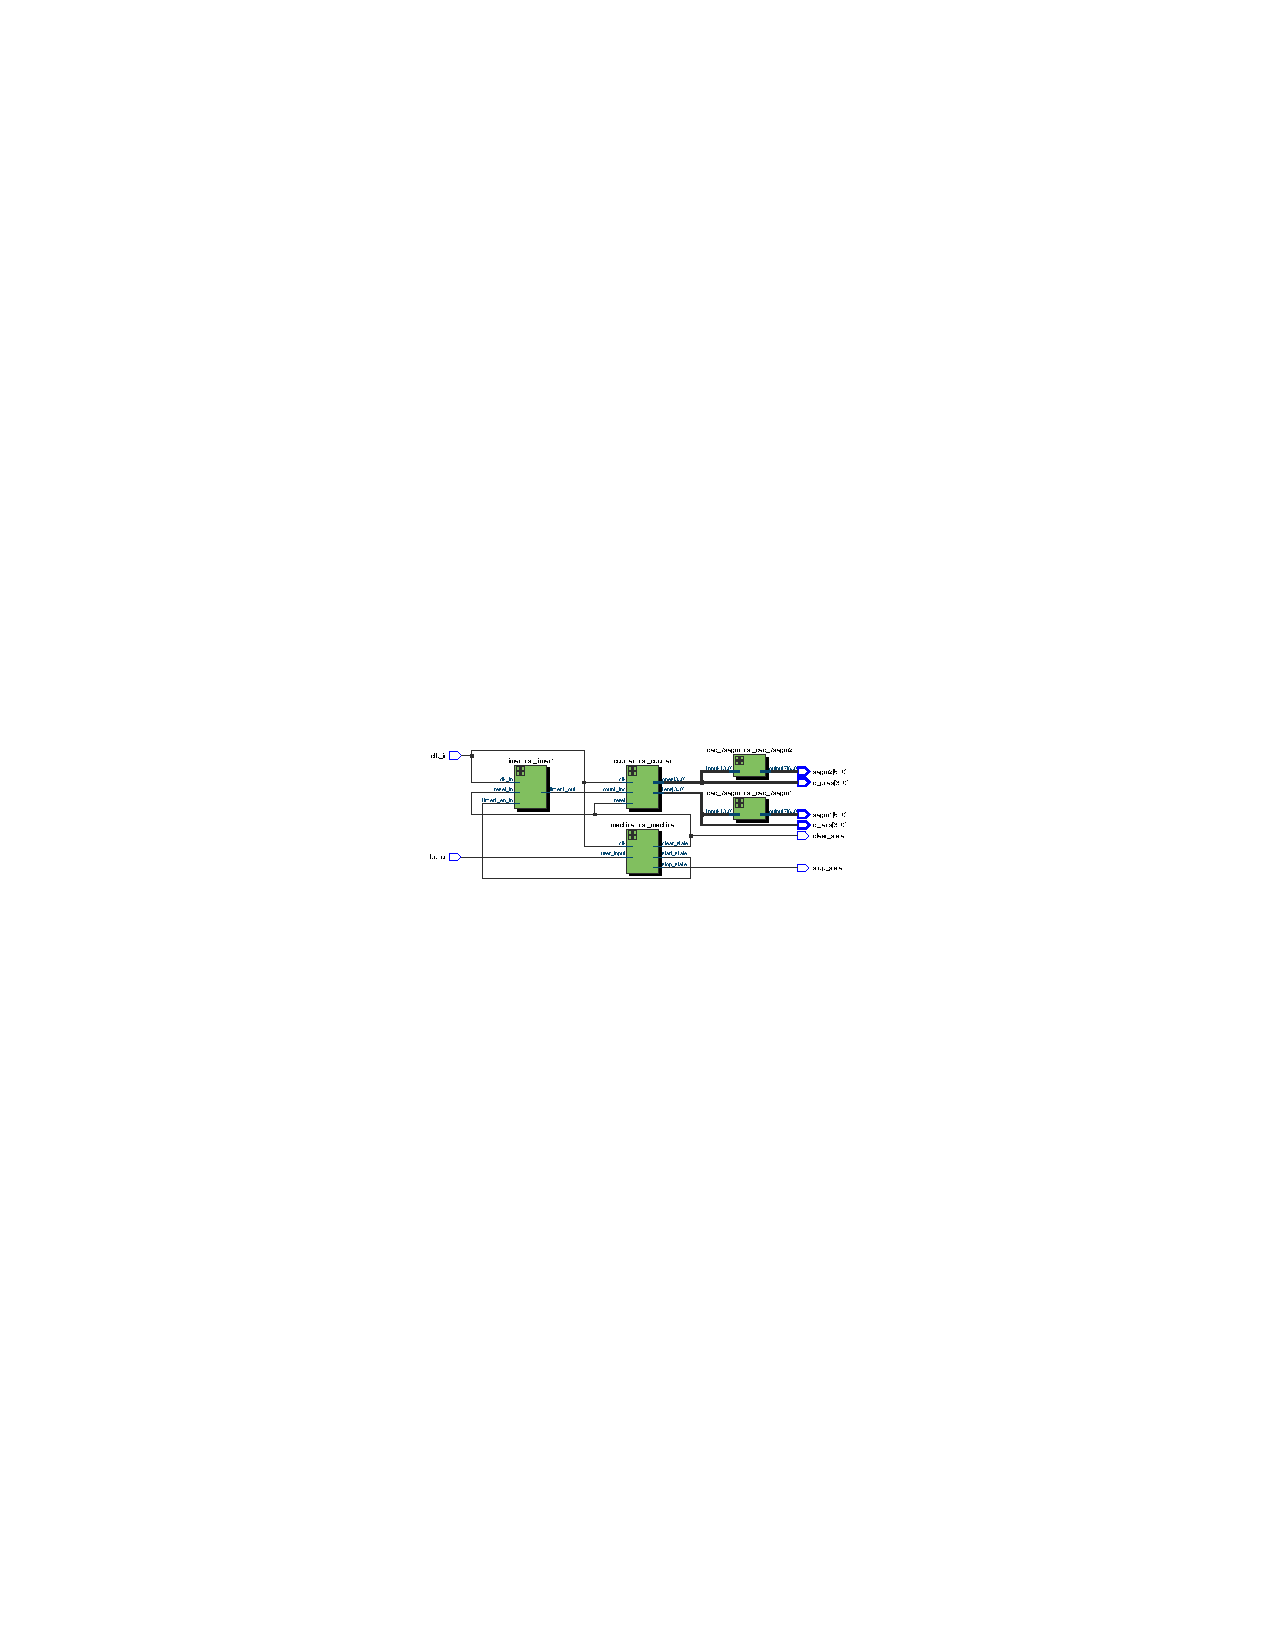
\includegraphics[clip,width=0.85\textwidth]{stopwatch.pdf}
	
	\section{Stavový automat}
	Stavový automat byl navržen dle přiloženého obrázku. Je vytvořen tak, aby vstup byl ošetřen a nedocházelo k několika přechodům během 1 stisku tlačítka. Bylo tak zamezeno náhodnému přepínání. Při stavech \uv{s0} a \uv{s1} je aktivní výstup \uv{stop\_state}, při stavech \uv{s2} a \uv{s3} je aktivní výstup \uv{clear\_state} a pouze při stavu \uv{s4} je aktivní výstup \uv{start\_state} tak, aby okamžitě při stisku tlačítka pro zastavení opravdu došlo k zastavení a ne až po stisku.

	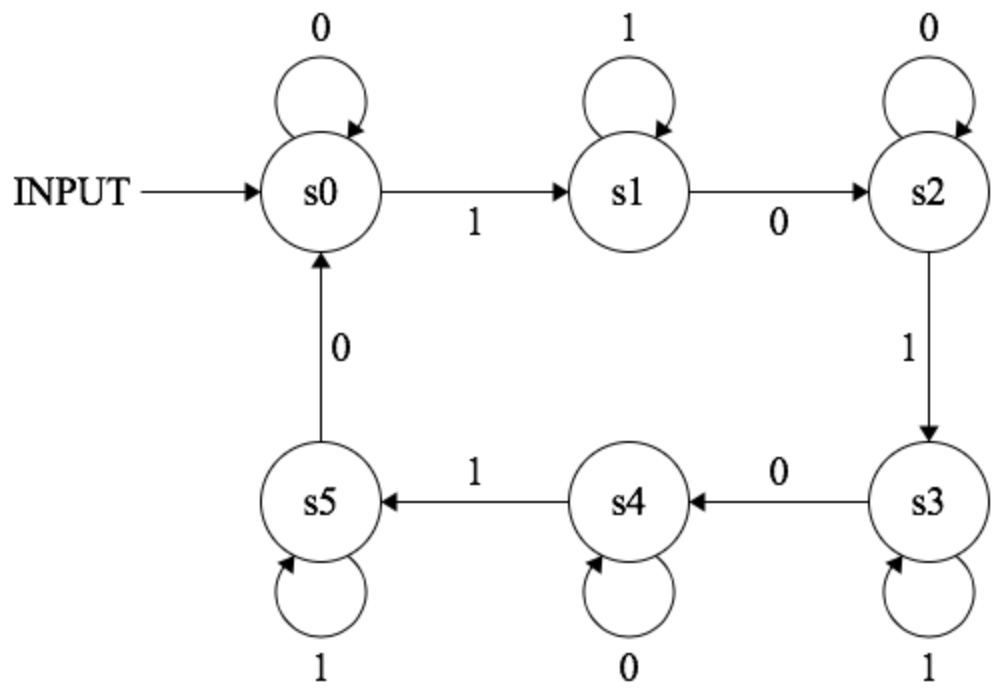
\includegraphics[clip,width=0.5\textwidth]{machine.png}
	
	\section{Detekce délky stisknutí tlačítka}
	Detekce délky stisknutí tlačítka byla již obtížnější část úlohy. Jako vstupy jsou v tomto bloku využity \uv{stop\_state} a \uv{clear\_state} z minulého bloku pro korektní nulování a funkcionalitu. Dále je zde uživatelský vstup tlačítko 2.
	Při držení tlačítka 2 je spuštěný časovač. Pokud časovač běží déle než 2 sekundy, tak je výstup časovače v logické 1. Tato hodnota a její inverze se uloží do klopných obvodů D a jsou tak jedinými výstupy tohoto bloku. Ty jsou navíc podmíněny stavem \uv{stop\_state}, tedy pokud není v požadovaném stavu, tak je vždy v logické 0. Zároveň je výstup ošetřen pomocí tlačítka, tedy dokud je stisknuté tlačítko, výstup je také v logické 0.
	
	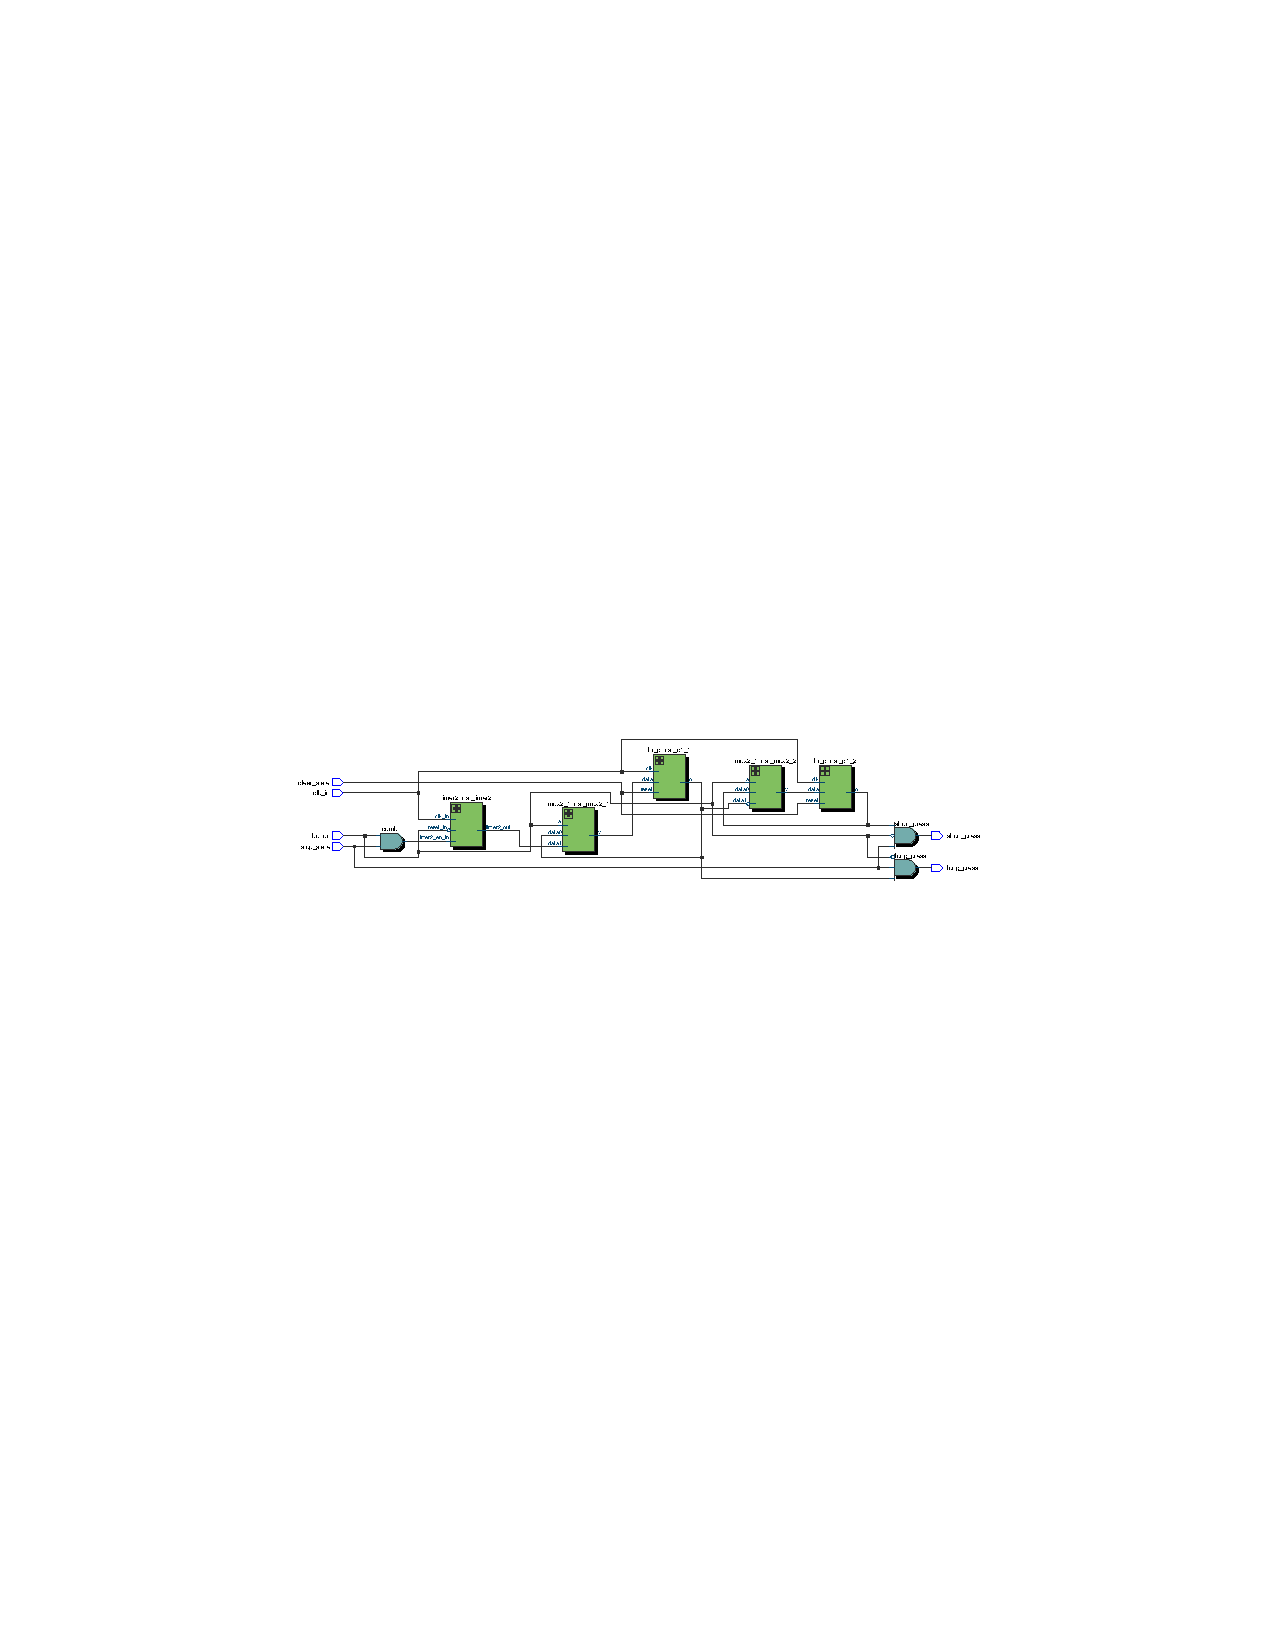
\includegraphics[clip,width=0.9\textwidth]{hold_detector.pdf}
	
	\section{Uložení a zobrazení hodnoty}
	Tento blok má jako vstup nadetekovanou délku stisku tlačítka 2 a aktuální hodnotu čítače z prvního bloku, tj. bloku realizují pouze stopky. Hodnoty čítače jsou přivedeny do multiplexoru, který je přepínán zjištěnou délkou stisku. Hodnoty jsou následně uloženy pomocí klopných obvodů D. Obdobně to funguje v případě zobrazení uložené hodnoty, ta se pouze uloží do dalších klopných obvodů D. Jejich výstup je následně přiveden do dekodéru a poté do segmentovek pro zobrazení hodnoty.
	
	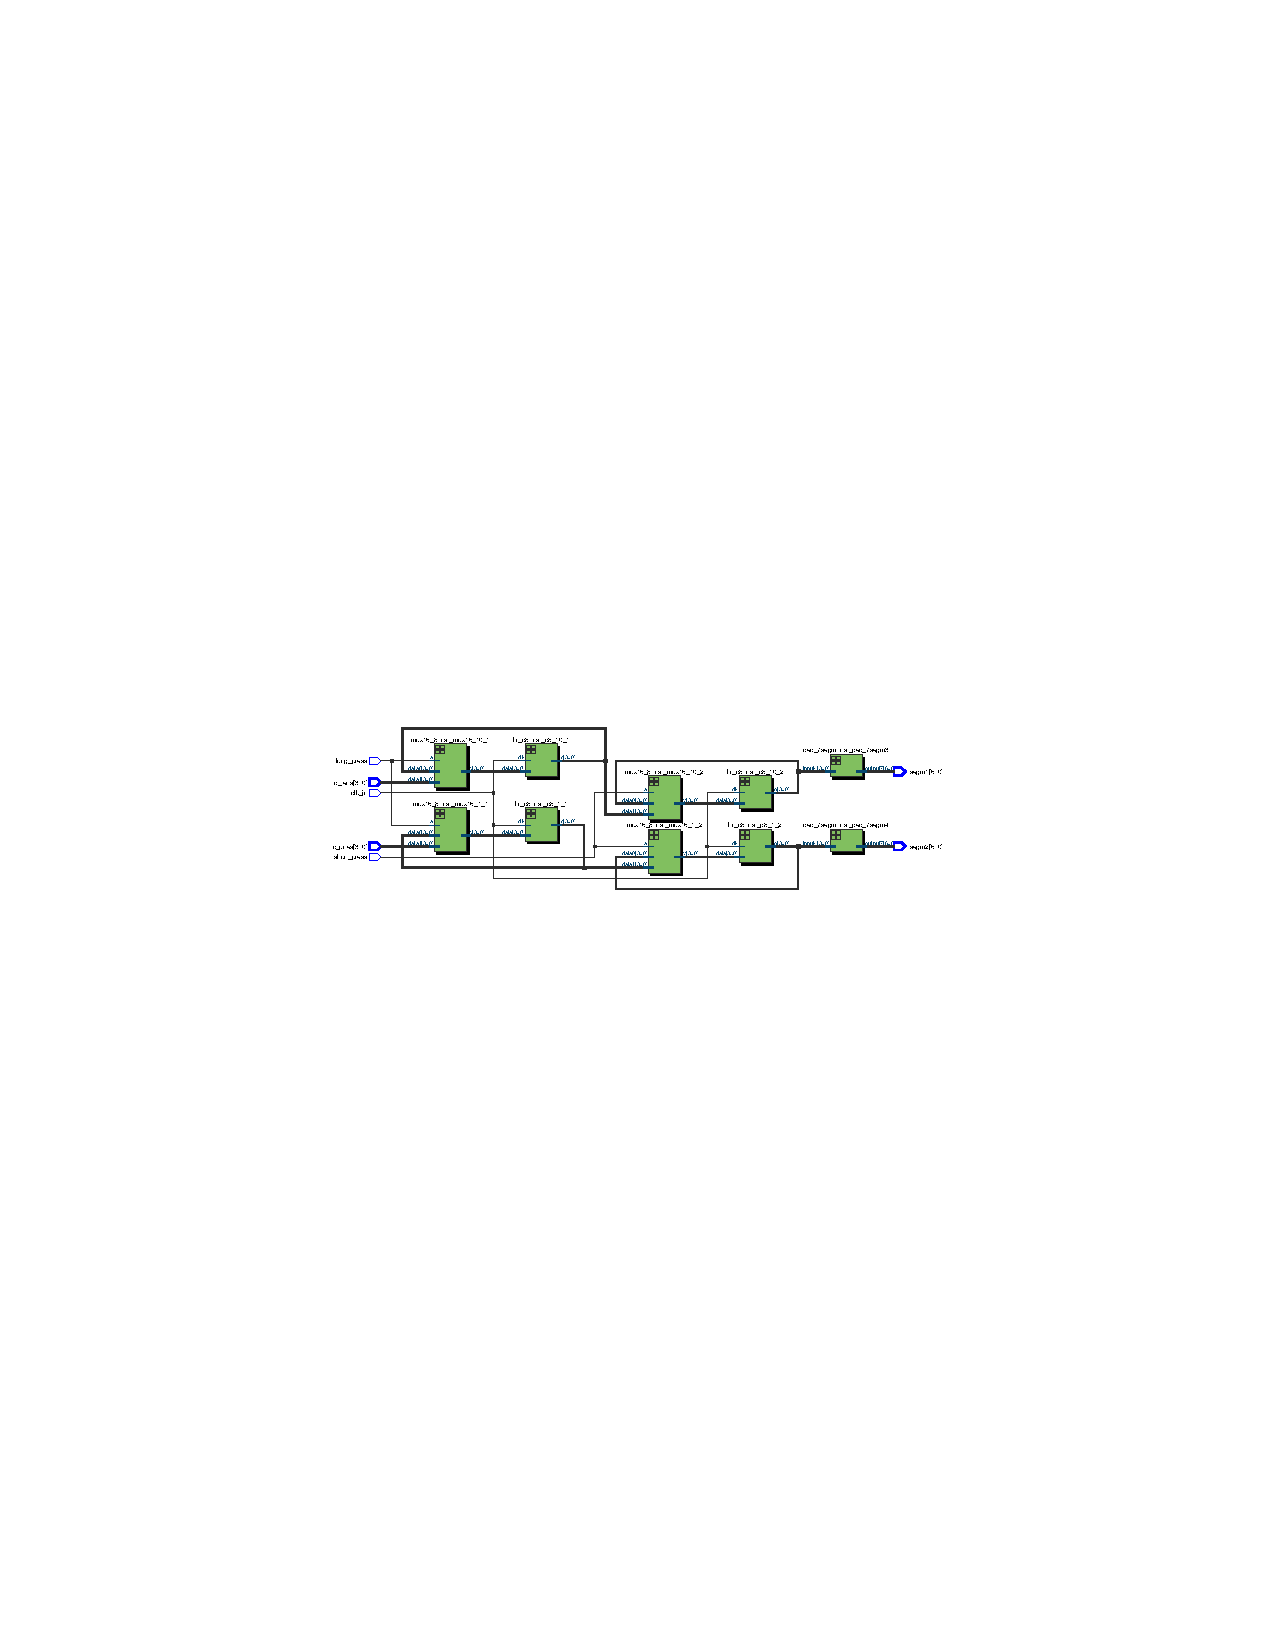
\includegraphics[clip,width=0.9\textwidth]{display_memory.pdf}
\end{document}